\documentclass[10pt,twocolumn,twoside,final]{IEEEtran}

% cite package, to clean up citations in the main text. Do not remove.
\usepackage{cite}
\usepackage{lastpage,fancyhdr,graphicx}
\usepackage{amssymb,amsmath}
\usepackage{mathtools}

% Remove brackets from numbering in List of References
\makeatletter
\renewcommand{\@biblabel}[1]{\quad#1.}
\makeatother

% *** SUBFIGURE PACKAGES ***
\ifCLASSOPTIONcompsoc
  \usepackage[caption=false,font=footnotesize,labelfont=sf,textfont=sf]{subfig}
\else
  \usepackage[caption=false,font=footnotesize]{subfig}
\fi

\begin{document}

\title{Effective Dynamic Models of Metabolic Networks}


% author names and affiliations
% use a multiple column layout for up to three different
% affiliations
\author{\IEEEauthorblockN{Michael Vilkhovoy\IEEEauthorrefmark{1},
Mason Minot\IEEEauthorrefmark{2},
Jeffrey D. Varner\IEEEauthorrefmark{1}}\\
\IEEEauthorblockA{\IEEEauthorrefmark{1}School of Chemical Engineering, Purdue University, West Lafayette, IN 47907 USA}
\IEEEauthorblockA{\IEEEauthorrefmark{2}School of Chemical and Biomolecular Engineering, Cornell University, Ithaca, NY 14850 USA}
\thanks{Manuscript received December 1, 2012; revised September 17, 2014.
Corresponding author: J. Varner (email:jdvarner@purdue.edu).}}

\maketitle

\begin{abstract}
Mathematical models of biochemical networks are useful tools to understand and ultimately predict how cells utilize nutrients to produce valuable products.
Hybrid cybernetic models in combination with elementary modes (HCM EM) provides a route to model cellular metabolism.
However, this framework is limited to smaller networks due to the computational cost of calculating elementary modes and a high number of solutions for large networks.
In this study, we developed a hybrid cybernetic model in combination with flux balance analysis (HCM FBA) modes instead of elementary modes.
Flux balance analysis provides a sufficient number of modes (metabolic options) for the network to estimate experimental observations.
We show HCM FBA has comparable model performance to HCM EM for a hypothetical proof of concept metabolic network and for a reduced anaerobic \textit{E. coli} network.
HCM FBA was applied to a larger metabolic network where 29 FBA modes were computed, in contrast to over 66,000 elementary modes.  A sensitivity analysis was performed to reduce the number of FBA modes from 29 to 5. This reduction maintained a robust model performance to fit experimental observations.

\end{abstract}


\begin{IEEEkeywords}
Dynamic metabolic models, flux balance analysis, cybernetic models
\end{IEEEkeywords}

\section{Introduction}
Metabolic networks for simple organisms such as \textit{E. coli} contain thousands of reactions that are highly interconnected.
These organisms have the potential to be engineered to produce valuable products.
Mathematical models of biochemical networks are useful tools to understand and ultimately predict how cells utilize nutrients to produce valuable products.
Traditionally, Monod kinetics have been used as unstructured models to describe cell growth, substrate consumption, and product formation, but fail to account for intracellular metabolism\cite{shuler_book}.
Structured modeling approaches have made great progress to describe metabolic pathways including elementary mode analysis (EM)\cite{2006_vonKamp_Metatool}, metabolic flux analysis (MFA), flux balance analysis (FBA)\cite{2010_orth_NatBiotech}, dynamic FBA (DFBA) \cite{1994_varma_palsson_ApplEnvMicro,2002_Mahadevan_BiophysJ}, and hybrid cybernetic modeling (HCM) \cite{2008_kim_varner_ramkrishna_BiotechProg}.

Convex and constraints based analysis methods, such as EM, FBA and MFA,
describe intracellular metabolism using the stoichiometry of the biochemical networks and the pseudo-steady state assumption \cite{2010_orth_NatBiotech}.
EM analysis is a powerful tool to decompse a metabolic network into independent minimal pathways that are stoichiometrically and thermodynamically feasible.
However, elementary mode calculations are computational expensive and infeasible for genome scale networks\cite{2004_lee_varner_ko_ieee}.
FBA is frequently used to study genome-scale networks\cite{2010_orth_NatBiotech} and often results in good approximations for yields, however it fails to estimate intracellular metabolism due to its underdetermined solution space.
Compared with FBA, MFA has good estimations of intracellular metabolism, but is dependent on experimental data.
Just like FBA, HCM approaches cell metabolism as a resource allocation problem towards a specified objective.
But HCM has multiple pathways to select from (elementary modes) and can use a combination of modes to direct its resources through the cell.
HCM has been shown to have comparable internal flux estimations to MFA and is able to estimate dynamic external fluxes with respect to experimental observations \cite{2008_kim_varner_ramkrishna_BiotechProg}.
DFBA is able to account for dynamic external fluxes but fails to incorporate the regulatory processes involved with HCM without the use of boolean rules\cite{2001_covert_schilling_palsson}.
Despite the advantages of HCM, it is restricted to small networks due to the exponential increase of the number of elementary modes for large networks.
Recent work has been done to reduce the number of elementary modes by lumping modes into groups using complex weighting schemes and experimental data\cite{2010_song_ramkrishna}, however, HCM is still limited by EM decomposition.

In this study, we developed a hybrid cybernetic model in combination with flux balance analysis modes instead of elementary modes.
We show HCM FBA has comparable model performance to HCM EM for a hypothetical metabolic network and a reduced anaerobic \textit{E. coli} network.
HCM EM and HCM FBA were then applied to a large metabolic network.
The number of elementary modes made it impractical to model with HCM EM, but HCM FBA was computationally feasible and performed well with respect to experimental observations.
Taken together, HCM FBA has comparable model performace to HCM EM and may be potentially applied to genome-scale networks which was a shortcoming of HCM EM.


\begin{figure}[!t]\centering
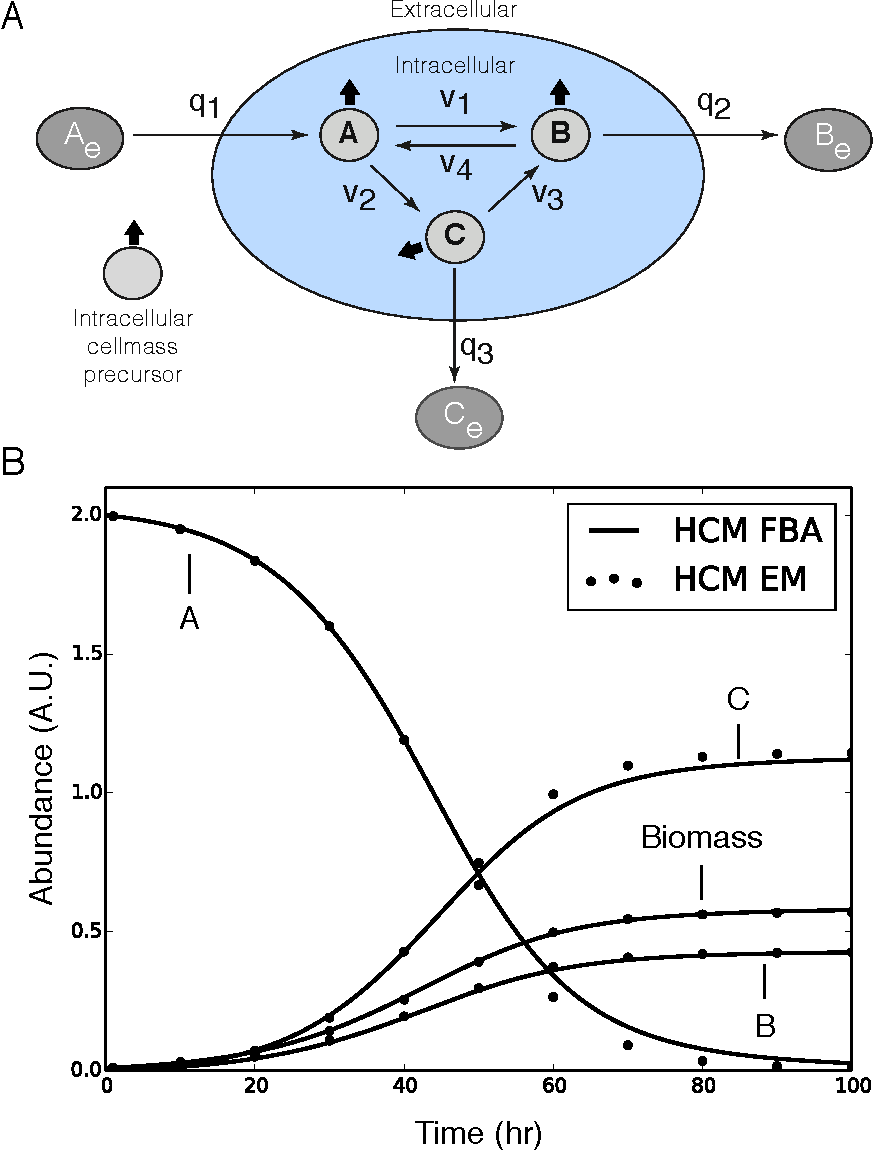
\includegraphics[width=0.40\textwidth]{./figs/Fig-1-GeneralModel-Results.pdf}
\caption{A: Proof of concept metabolic network with six metabolites and seven reactions.
Intracellular cellmass precursors $A,B$ and $C$ are balanced (no accumulation) while the extracellular metabolites ($A_{e},B_{e}$ and $C_{e}$) are not balanced (can accumulate). The blue-oval denotes the cell boundary, where $q_{j}$ denotes the jth flux across the boundaries ([mmol/gdw-hr]) and $v_{k}$ denotes the kth intracellular flux. B: Simulation of the extracellular metabolites using the FBA hybrid cybernetic approach (solid line) versus elementary modes (points) for the proof of concept metabolic network. FBA modes have comparable model performance compared to elementary modes.
}\label{fig:model-fitting}
\end{figure}

\section{Results}
The performance of the HCM FBA approach was equivalent to HCM EM for a proof of concept metabolic network (Fig. \ref{fig:model-fitting}).
The proof of concept network, consisting of six metabolites and seven reactions (Fig. \ref{fig:model-fitting}A), generated three FBA and six elementary modes.
Using the elementary modes and synthetic parameters, we generated test data from which we estimated the HCM FBA model parameters.
The best fit HCM FBA model replicated the synthetic data (Fig. \ref {fig:model-fitting}B).
The HCM EM and HCM FBA kinetic parameters were not quantitatively identical, but had similar orders of magnitude;
the FBA approach had three fewer modes, thus you would not expect identical parameter values.
Taken together, the HCM FBA approach replicated synthetic data generated using HCM EM, despite having three fewer modes.
Next, we tested the ability of HCM FBA to replicate experimental data.

%In the case, we demonstrated that HCM FBA has comparable model performance to a published HCM EM model \cite{2008_kim_varner_ramkrishna_BiotechProg}.
%and elementary modes reported
%The kinetic parameters of HCM FBA were varied to fit the same experimental observations.
%HCM FBA has 17 kinetic parameters while HCM EM has 21 kinetic parameters and both models resulted in similar fits to the experimental data .
%HCM FBA had a better fit on lactate than HCM EM by 35.6\% on the
%However, HCM EM had a lower residual standard error on the overall performance by 4.5\%.
%However, ZZZ has shown that the EM algorithm has exponential runtime complexity [REFHERE].
%Thus, HCM EM may not be possible for large networks, but HCM FBA will not suffer from this shortcoming.
%In the case, we demonstrated that HCM FBA is applicable for larger metabolic networks where elementary mode calculations increase exponentially.

The performance of HCM FBA was equivalent to HCM EM for a small model of anaerobic \textit{E. coli} metabolism (Fig. \ref{fig:ecoli}, left).
The anaerobic \textit{E. coli} network, consisting of 12 reactions and 19 metabolites, generated nine elementary and seven FBA modes.
HCM EM cellmass, glucose and fermentation product trajectories were generated
using these elementary modes and kinetic parameters reported by Kim et al. \cite{2008_kim_varner_ramkrishna_BiotechProg},
where the experimental data was taken from ZZZ et al. [REFHERE] (Fig. \ref{fig:ecoli}A, dashed).
We estimated the HCM FBA model parameters from the experimental measurements using simulated annealing.
Overall, HCM FBA performed only 5\% worse than HCM EM (Fig. \ref {fig:ecoli}A, solid), despite having two fewer modes and four fewer parameters (17 versus 21 parameters).
Taken together, these results suggested HCM FBA is an alternative to HCM EM even for cases when elementary modes can be easily calculated.

\begin{figure}[!t]\centering
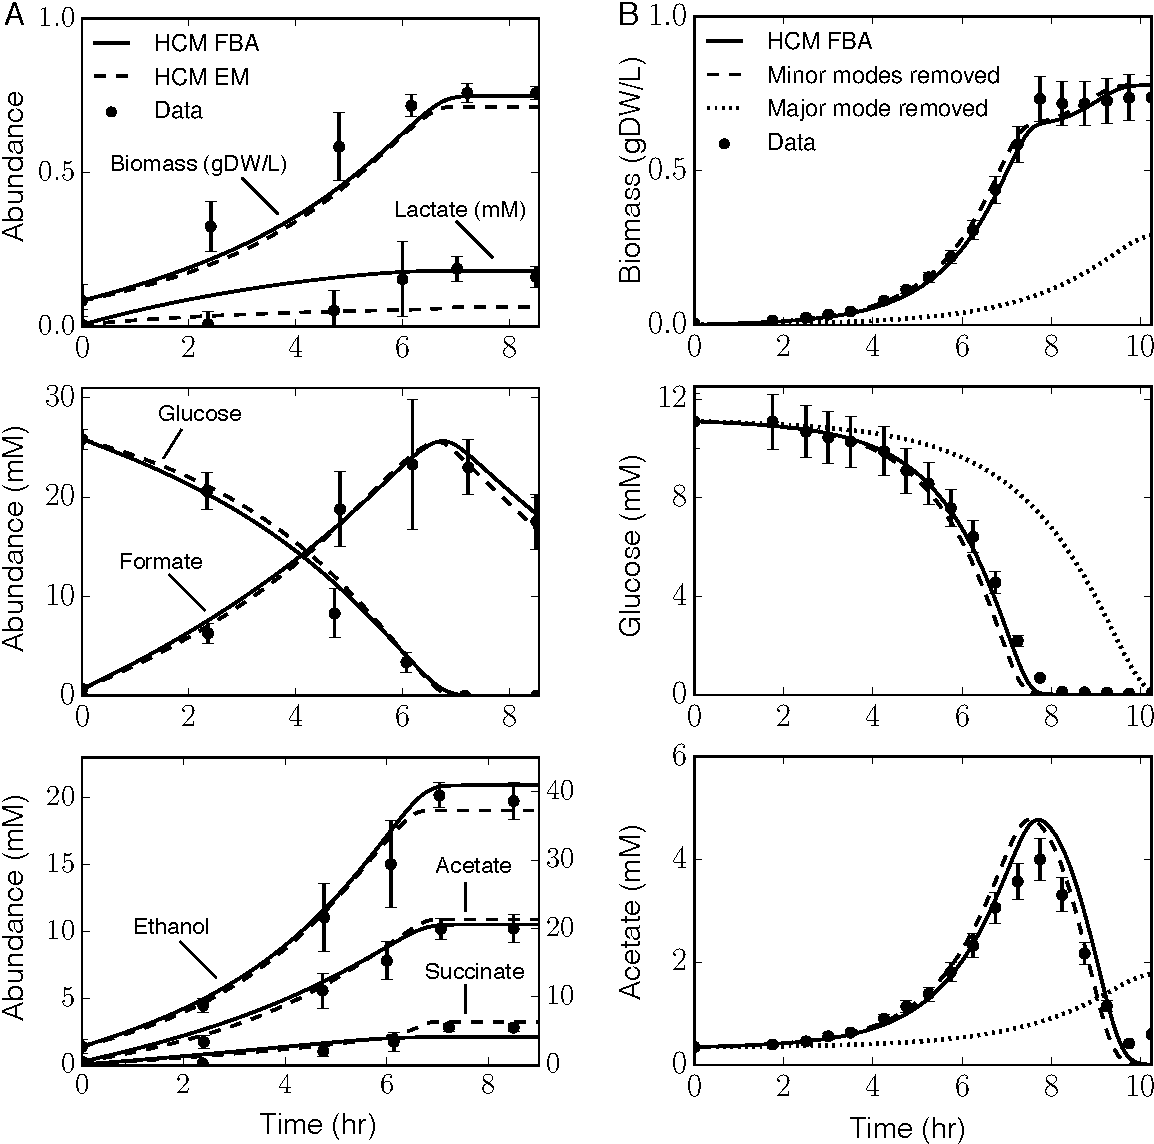
\includegraphics[width=0.48\textwidth]{./figs/Fig-2-Ecoli-SimulationResults.pdf}
\caption{A: Batch anaerobic \textit{E. coli} fermentation data versus simulation of the hybrid cybernetic model with FBA modes (solid line) and elementary modes (dashed line). (Experimental data from Kim et. al (2008)\cite{2008_kim_varner_ramkrishna_BiotechProg} with error bars representing 90\% confidence intervals.) B: Batch aerobic \textit{E. coli} fermentation data of glucose, acetate and cell density measurements versus simulation of the hybrid cybernetic model with FBA modes (solid line). Model performance is shown when minor modes (dashed) and a major mode (dotted) is removed from HCM FBA. (Experimental data from Varma \& Palsson (1994)\cite{1994_varma_palsson_ApplEnvMicro} with assumed 10\% error bars).}
\label{fig:ecoli}
\end{figure}

HCM FBA outperformed HCM EM for a large model of aerobic \textit{E. coli} metabolism (Fig. \ref{fig:ecoli}, right).
An \emph{E. coli} metabolic network, consisting of 60 metabolites and 110 reactions, was constructed from literature \cite{2007_schuetz_etal_MolSysBio,2006_Palsson_model}.
Elementary mode decomposition of this network was not feasible; we generated $>$ 150,000 elementary modes before prematurely terminating the calculation.
Conversely, flux balance analysis generated only 29 modes for the same network.
HCM FBA model parameters were estimated from cellmass, glucose and acetate measurements generated by Palsson and coworkers \cite{1994_varma_palsson_ApplEnvMicro} (Fig. \ref{fig:ecoli}B, solid).
HCM FBA captured glucose consumption, cellmass formation and the switch between acetate production and consumption following glucose exhaustion.
Taken together, the aerobic \textit{E. coli} results demonstrated that HCM FBA was able to describe cell growth, including the switch between glucose and acetate consumption,
for a network that was infeasible to decompose using elementary modes.
However, it was unclear whether all 29 FBA modes were required to capture the experimental data.

Variance based sensitivity of aerobic \textit{E. coli} metabolism identified which FBA modes that were essential to biomass yield (Fig. \ref{fig:sensitivity}).
The analysis calculated the total order sensitivity indicies of all the kinetic parameters and enzyme initial conditions.
We used the sensitivity results as a simple systematic method to eliminate FBA modes to give the smallest number needed while maintaining good model performance.
Five FBA modes were determined to be significant by an arbitrary threshold of 0.00218.
The remaining 24 FBA modes were identified to be minor modes and insignificant.
The removal of the major mode, representing aerobic growth, (Fig, \ref{fig:ecoli}B, dotted)
was detrimental to model performance, whereas the removal of the minor modes (dashed line) had little effect.

\begin{figure*}[!t]\centering
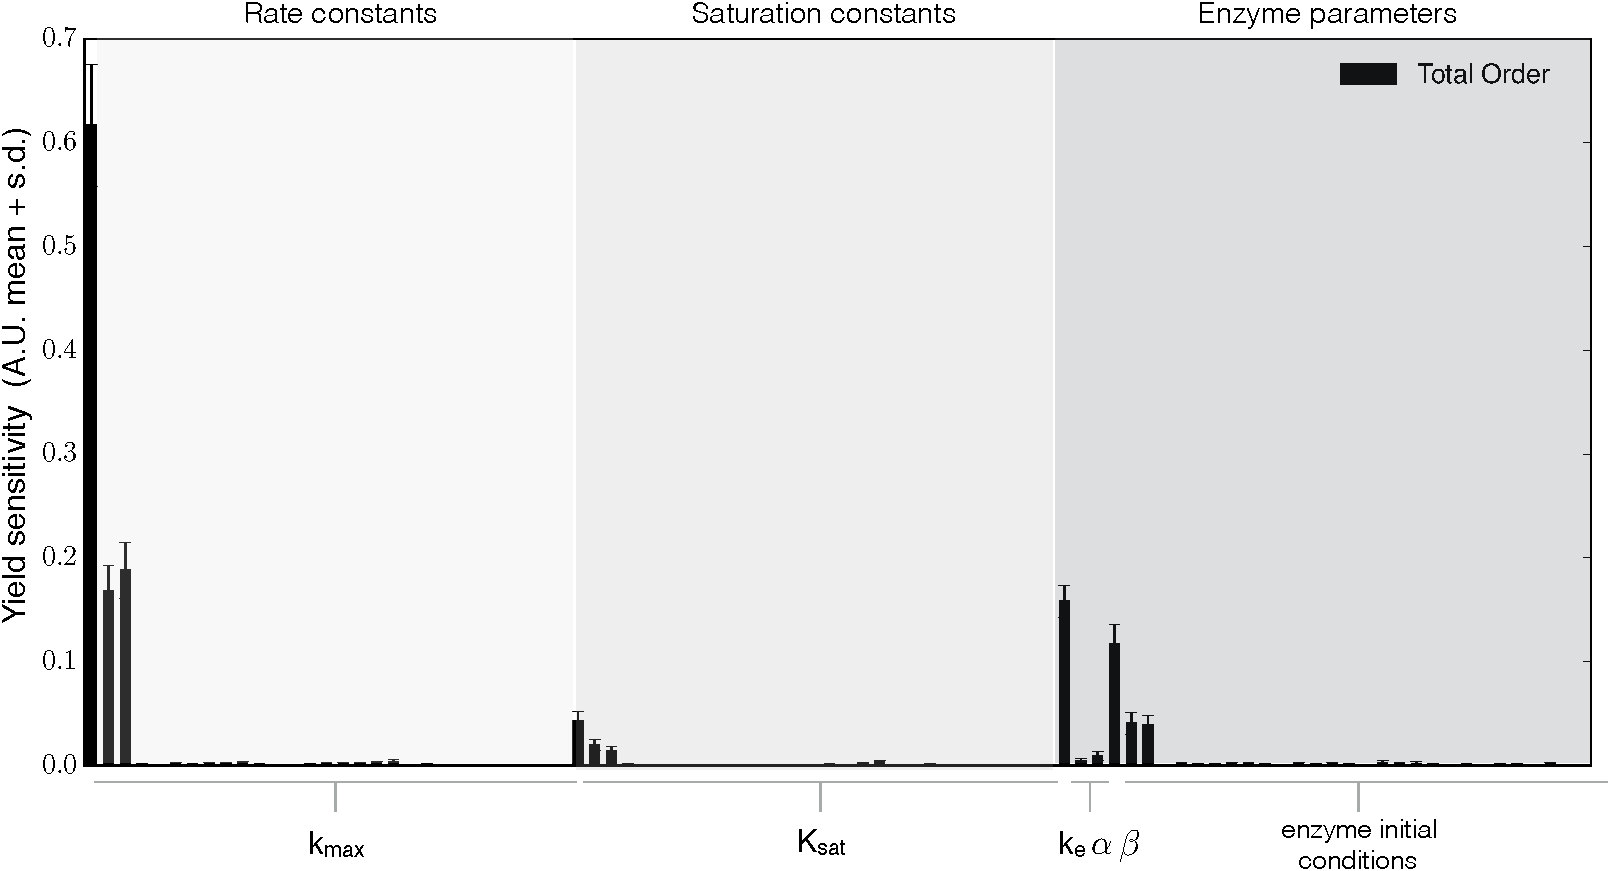
\includegraphics[width=0.80\textwidth]{./figs/Fig-3-Sensitivity-Results.pdf}
\caption{Total order variance based sensitivity analysis on biomass yield from glucose and acetate. Sensitivity indicies computed for rate constants, saturation constants and enzyme parameters. The most critical parameters are associated with mode 1 representing aerobic growth. (Error bars represent 95\% confidence intervals).
}
\label{fig:sensitivity}
\end{figure*}


\section{Discussion}
In this study, we developed a hybrid cybernetic model in combination with flux balance analysis modes instead of elementary modes.
First, we showed HCM FBA can have comparable model performance to HCM EM for a proof of concept metabolic network.
This judgement is based on the quality of fit of the model simulation to the observations.
Next, HCM FBA model performance was compared to an established HCM EM model\cite{2008_kim_varner_ramkrishna_BiotechProg} for an anaerobic culture of \textit{E. coli}.
HCM FBA had comparable fits to HCM EM on the fermentation data and a slightly better fit on lactate measurements.
Finally, HCM was applied to a larger metabolic network where 29 FBA modes were computed, in contrast to over 66,000 elementary modes.
HCM FBA was shown to have robust model performance only requiring 5 of the 29 FBA modes (selected by the sensitivity analysis) to fit experimental observations.

The hybrid cybernetic model is formulated to maximize substrate uptake based on cybernetic arguments.
Towards this objective, HCM uses a combination of modes to describe both the external and internal fluxes.
The internal fluxes still follow the pseudo steady state approximation applied in FBA, but HCM uses a combination of pathways.
HCM EM has been shown to have comparable internal flux estimates to MFA results\cite{2008_kim_varner_ramkrishna_BiotechProg}, this has not been shown for HCM FBA.
The HCM framework has been shown to predict dynamic external fluxes using both elementary and FBA modes.
While DFBA already has the capacity to estimate dynamic external fluxes, it requires \textit{a priori} knowledge and boolean rules to capture the diauxic phenomena \cite{1994_varma_palsson_ApplEnvMicro,2002_Mahadevan_BiophysJ,2001_covert_schilling_palsson}.
HCM overcomes this by incorparting the regulatory processes of substrate utilization based on its cybernetic arguments.
HCM EM has good model performance for reduced networks, but is impractical for larger networks.
HCM EM has been applied to a network with 67 reactions, requiring the elementary modes to be lumped into groups by complex weighting schemes and relying on experimental data\cite{2010_song_ramkrishna}.
A shortcoming of the HCM EM framework is that EM calculations are computationally expensive and the number of modes exponentially increases for larger networks \cite{2004_lee_varner_ko_ieee}.
In contrast, FBA does not have the computational burden associated with calculating elementary modes.
FBA is frequently used to study genome-scale networks\cite{2010_orth_NatBiotech} and can be used to generate modes for the HCM framework.
This opens up the possibility of genome scale cybernetic models.

HCM FBA provides a practical and feasible approach to model large networks where elementary modes fail.
The disadvantage of HCM FBA is it requires \textit{a priori} knowledge of the inputs into the metabolic network.
FBA modes do not have the thorough information as elementary modes, but provide sufficient pathways to model experimental observations.
%HCM FBA may also be applied to mammalian networks, as long as FBA accounts for compartmentalization within mammalian systems.

\section{Materials and Methods}
The HCM FBA approach is a modification of the HCM EM strategy of Kim et al. \cite{2008_kim_varner_ramkrishna_BiotechProg}. However, unlike HCM EM, we replaced elementary modes with flux balance analysis solutions. The abundance of extracellular species $i$ ($x_{i}$), the pseudo enzyme $e_{l}$ and cellmass are governed by:
\begin{eqnarray}\nonumber
	\frac{dx_{i}}{dt}  & = &  \sum_{j = 1}^{\mathcal{R}}\sum_{l = 1}^{\mathcal{L}}\sigma_{ij}z_{jl}r_{l}\left(\mathbf{e},\mathbf{k},\mathbf{x}\right)c \qquad{i=1,\hdots,\mathcal{M}}\\\nonumber
  \frac{de_{l}}{dt}  & = & \alpha_{l} + r_{E,l}\left(\mathbf{k},\mathbf{x}\right)u_{l} - \left(\beta_{l}+r_{G}\right)e_{l} \qquad l=1,\hdots,\mathcal{L} \\\nonumber
  \frac{dc}{dt} & = & r_{G}c
\end{eqnarray}
where $\mathcal{R}$ and $\mathcal{M}$ denote the number of reactions and extracellular species in the model, and $\mathcal{L}$ denotes the number of FBA modes.
The quantity $\sigma_{ij}$ denotes the stoichiometric coefficient for species $i$ in reaction $j$ and $z_{jl}$ denotes the normalized flux for reaction $j$ in mode $l$.
If $\sigma_{ij}>0$, species $i$ is produced by reaction $j$,
if $\sigma_{ij}<0$, species $i$ is consumed by reaction $j$, while $\sigma_{ij} = 0$ indicates species $i$ is not connected with reaction $j$.
Extracellular species balances were subject to the initial conditions $\mathbf{x}\left(t_{o}\right) = \mathbf{x}_{o}$ determined from experimental data.
The term $r_{l}\left(\mathbf{e},\mathbf{k},\mathbf{x}\right)$ denotes the specific rate of flux through mode $l$, and was written as the product of a kinetic term ($\bar{r}_{l}$) and a cybernetic control variable governing enzyme activity. Flux through each mode was catalyzed by a pseudo enzyme $e_{l}$, where enzyme $e_{l}$ was synthesized at the regulated specific rate $r_{E,l}\left(\mathbf{k},\mathbf{x}\right)$ and constitutively at the rate $\alpha_{l}$. The term $r_{E,l}$ denotes the specific rate enzyme synthesis for enzyme $l$, and $u_{l}$ denotes the cybernetic variable controlling the synthesis of enzyme $l$. The term $\beta_{l}$ denotes the rate constant governing enzyme degradation, and $r_{G}$ denotes the growth rate through all modes.
The specific rate of flux through an FBA mode, and the specific rate of enzyme synthesis were modeled using saturation kinetics.
All enzyme initial conditions were set to 0.9 for the anaerobic case, and 0.8 for the aerobic case.
Lastly, cellmass was produced at the specific growth rate:
\begin{equation}
	r_{G}  = \sum_{l = 1}^{\mathcal{L}}z_{\mu l}r_{l}\left(\mathbf{e},\mathbf{k},\mathbf{x}\right)
\end{equation}
where $z_{\mu l}$ denotes the growth flux $\mu$ through mode $l$.
The cybernetic control variables $u_{l}$ and $v_{l}$, which control the synthesis and activity of each enzyme respectively, were given by:
\begin{align*}
	u_{l}  = \frac{z_{sl}\bar{r}_{l}}{\sum\limits_{l = 1}^{\mathcal{L}}z_{sl}\bar{r}_{l}} && v_{l} = \frac{z_{sl}\bar{r}_{l}}{\max\limits_{\mathbf{l}} z_{sl}\bar{r}_{l}}
\end{align*}
where $z_{sl}$ denotes the uptake flux of substrate $x$ through mode $l$.
In the anaerobic case we followed the assumption of Kim et al.\cite{2008_kim_varner_ramkrishna_BiotechProg},
that formate decomposition occurs only outside the network (applicable for strain GJT001).
Therefore its enzyme activity was assumed to be at its maximum level of unity.
The reaction rate for formate was also modified following Kim et al.\cite{2008_kim_varner_ramkrishna_BiotechProg}. All numerical simulations were conducted in Julia version 0.4.2, a high-level, high performance dynamic programming language \cite{Julia}. Species balances were solved using a Sundials \cite{Sundials} wrapper for julia.

\noindent\subsubsection*{Elementary Mode and Flux Balance Analysis}
Elementary modes were calculated using METATOOL 5.1 \cite{2006_vonKamp_Metatool}.
FBA modes were defined as the solution flux vector through the network connecting substrate uptake to cellmass and extracellular product formation.
The FBA problem was formulated as:
\begin{equation}
 \begin{multlined}
	\qquad \qquad \qquad \max_{\boldsymbol{w}}{} \! \left( w_{obj} = \mathbf{\theta}^T \boldsymbol{w} \right) \\
	\mathrm{Subject \; to:}
	 \; \; \mathbf{S}\mathbf{w}=\mathbf{0} \\
\alpha_i \leq w_i \leq \beta_i  \qquad
 \end{multlined}
\end{equation}
where $\mathbf{S}$ denotes the stoichiometric matrix, $\mathbf{w}$ denotes the unknown flux vector, $\boldsymbol{\theta}$ denotes the objective selection vector
and $\alpha_i$ and $\beta_i$ denote the lower and upper bounds on flux $w_{i}$, respectively.
The flux balance analysis problem was solved using the GNU Linear Programming Kit, GLPK version 4.52 \cite{GLPK}.
For each FBA mode, the objective was to maximize either the growth rate, or the specific rate of byproduct formation from a specified starting substrate.
Multiple FBA modes were calculated for each objective flux by allowing the oxygen and nitrate uptake rates to be either zero or maximal.
For aerobic metabolism, the specific oxygen and nitrate uptake rates were constrained to allow a maximum flux of 10 mM/gDW$\cdot$hr and 0.05 mM/gDW$\cdot$hr, respectively.
Each flux vector was normalized by the growth flux, or by the specified objective flux.

\subsubsection*{Global Sensitivity Analysis}
Variance based sensitivity analysis was used to estimate which FBA modes were critical to model performance.
The performance function used in this study was the biomass yield on substrate.
Candidate parameter sets (N = 182,000) were generated using Sobol sampling by perturbing the best fit parameter set $\pm50\%$ \cite{SALib}.
Model performance, calculated for each of these parameter sets, was then used to estimate the total-order sensitivity coefficient for each model parameter.

\subsubsection*{Estimation of model parameters}
Model parameters were estimated by minimizing the difference between simulations and experimental measurements (squared residual):

\begin{equation}\label{eqn:objective-function}
	\min_{\mathbf{k}} \sum_{\tau=1}^{\mathcal{T}}\sum_{j=1}^{\mathcal{S}}\left(\frac{\hat{x}_{j}\left(\tau\right) - x_{j}\left(\tau,\mathbf{k}\right)}{\omega_{j}\left(\tau\right)}\right)^{2}
\end{equation}
where $\hat{x}_{j}\left(\tau\right)$ denotes the measured value of species $j$ at time $\tau$, $x_{j}\left(\tau,\mathbf{k}\right)$ denotes the simulated
value for species $j$ at time $\tau$, and $\omega_{j}\left(\tau\right)$ denotes the experimental measurement variance for species $j$ at time $\tau$.
The outer summation is with respect to time, while the inner summation is with respect to state. The model residual was minimized using simulated annealing.

% References -
\bibliographystyle{naturemag_noURL}
\bibliography{Paper_v1}

\end{document}
\grid
